\section{Fluid Mechanics}
\subsection{Kinematics}
\subsubsection{Coordinates}
\textbf{Lagrangian} $\underline{\boldmath{x}}(\underline{\boldmath{a}},t)$: The \textit{motion of individual particles} is studied; the position $\underline{\boldmath{x}}$ of a particle at time $t$ is related to its position at a reference point in time \underline{\boldmath{a}} (typically at $t=0$).
\newline
\newline
\textbf{Eulerian} $(\underline{\boldmath{x}},t)$: 
The \textit{'flow field' is considered as a whole} and the state of a fluid is described in terms of the values at a fixed location $\underline{\boldmath{x}}$ and at a fixed time $t$
\subsubsection{Velocity}
In Cartesian coordinates the velocity of a fluid particle at position $\underline{\boldmath{x}}(x,y,z)$ is given by:
\begin{center}
	$\underline{\boldmath{u}}(x,y,z) = u(x,y,z)\underline{\hat{i}} + v(x,y,z)\underline{\hat{j}} + w(x,y,z)\underline{\hat{k}}$
\end{center}
\subsubsection{Stagnation Points}
Stagnation points occur when the velocity vector $\underline{u}$ is equal to $\underline{0}$
\begin{align*}
	u = 0
	\\
	v= 0
	\\
	w= 0
\end{align*}
\subsubsection{Streamlines}
A streamline is a curve $C$ drawn at one point in time such that the fluid velocity vector $\underline{u}$ is tangent to $C$ at every point along $C$.
\begin{center}
	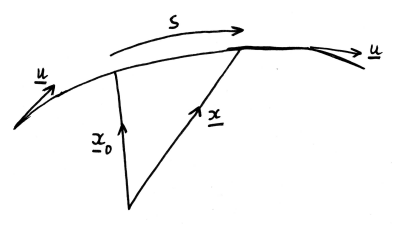
\includegraphics[width = 0.5\textwidth]{"Images/Streamline.png"}
\end{center} 
\begin{align*}
	\frac{d\underline{x}}{ds} = \underline{u}
	\\
	\\
	\frac{dx}{ds}=u , \frac{dy}{ds}=v ,  \frac{dz}{ds}=w
	\\
	\\
	\boxed{\frac{dx}{u}=\frac{dy}{v}=\frac{dz}{w}(= ds)}
\end{align*}

\subsubsection{Particle Paths}
Particle path is obtained by solving the initial value problem:
\begin{center}
		$\frac{d\underline{x}}{dt} = \underline{u}(\underline{x},t)$ , $\underline{x} = x_0$ at $t = 0$
		\\
		\begin{tabular}{|c|}
			\hline
			\\
				$\frac{dx}{dt} = u$ , $x(0)=x_0$
			\\ 
			\\
			$\frac{dy}{dt} = v$, $y(0)=y_0$
			\\
			\\
			$\frac{dz}{dt} = w$, $z(0)=z_0$
			\\
			\\
			\hline
		\end{tabular}
\end{center}

	
		


\subsubsection{Steady Flow}

\textbf{Steady Flow}: The flow velocity vector $\underline{u}$ is independent of time $t$
\newline
\textbf{Unsteady Flow}: $\underline{u}$ depends on $t$; the pattern of streamlines changes with $t$
\subsubsection{Convective Derivative}
The convective derivative tells us how a property changes \textit{as it moves with a flow}.
\\
\textbf{General}
\begin{center}
	\boxed{
		\frac{D\mathbf{*}}{Dt} =  \frac{\partial\mathbf{*}}{\partial t} + (\underline{u} \cdot \nabla)\mathbf{*}=\frac{\partial\mathbf{*}}{\partial t} + u\frac{\partial\mathbf{*}}{\partial x}+ v\frac{\partial\mathbf{*}}{\partial y} + w\frac{\partial\mathbf{*}}{\partial z}}
\end{center}
\textbf{Scalar}
\begin{center}
	\boxed{
		\frac{D\mathbf{\rho}}{Dt} =  \frac{\partial\mathbf{\rho}}{\partial t} + (\underline{u} \cdot \nabla)\mathbf{\rho} = \frac{\partial\mathbf{\rho}}{\partial t} + u\frac{\partial\mathbf{\rho}}{\partial x}+ v\frac{\partial\mathbf{\rho}}{\partial y} + w\frac{\partial\mathbf{\rho}}{\partial z}}
\end{center}
\textbf{Vector}
\begin{center}
	\boxed{
		\frac{D\mathbf{\underline{u}}}{Dt} =  \frac{\partial\mathbf{\underline{u}}}{\partial t} + (\underline{u} \cdot \nabla)\mathbf{\underline{u}}= \frac{\partial\mathbf{\underline{u}}}{\partial t} + u\frac{\partial\mathbf{\underline{u}}}{\partial x}+ v\frac{\partial\mathbf{\underline{u}}}{\partial y} + w\frac{\partial\mathbf{\underline{u}}}{\partial z}}
\end{center}
\subsubsection{Vorticity}
Vorticity \underline{$\omega$} is a measure of the local rotation of fluid particles in flow.
\\
\begin{center}
	\boxed{\underline{\omega} = \nabla \times \underline{u}}
\end{center}
\begin{center}
	$\nabla \times \underline{u} = \begin{vmatrix}
	\underline{i} & \underline{j} & \underline{k}\\ 
	\frac{\partial}{\partial x} & \frac{\partial}{\partial y} & \frac{\partial}{\partial z}\\
	u & v & w 
\end{vmatrix}$
\end{center}
\textbf{Irrotational Flow}:
\\
\begin{center}
	\boxed{\underline{\omega} = \underline{0}}
\end{center}
\subsubsection{Incompressible Flow}
\begin{center}
	\boxed{\nabla \cdot \underline{u} = 0}
\end{center}
	When this is true the convective derivative of the fluid density is zero:
	\begin{center}
		$\frac{D\rho}{Dt} = 0$
	\end{center}
\subsubsection{Velocity Potential}
For an irrotational flow the velocity can be described as the gradient of a scalar field known as the \textit{Velocity Potential}.
\begin{center}
	$\nabla \times \underline{u} = 0$
	\\
	The curl of the gradient of a scalar field is zero:
	\\
	$\nabla \times (\nabla \phi) = 0$
	\\
	$\underline{u} = \nabla\phi$
\end{center}
If the flow is also incompressible
\begin{center}
	$\nabla \cdot \underline{u} = 0$
	\\
	$\nabla \cdot (\nabla \phi) = 0$
	\\
	Therefore the velocity potential of an irrotational, incompressible flow satisfies Laplace's Equation:
	\\
	\boxed{\nabla^2 \phi = 0}
\end{center}
\subsubsection{Equipotential Surfaces}
Lines/surfaces of constant $\phi$ are \textit{equipotentials}.
\\
	The velocity potential can be considered a surface:
	\begin{center}
		$\phi(x,y,z)=c$
	\end{center}
	Let $\underline{a}$ be tangent to the surface, the derivative of $\phi$ in the direction of $\underline{a}$:
	\\
	\begin{center}
		$\underline{a}\cdot\nabla \phi = 0$
	\end{center}
	Because the derivative of a constant $c$ is zero: $\nabla \phi$ is normal to the surface.
	\begin{center}
		\boxed{\hat{\underline{n}}=\frac{\nabla \phi}{\vert\nabla \phi\vert} }
	\end{center}
\subsubsection{The Stream Function}
Considering incompressible two dimensional flow:
\begin{center}
	$\nabla \cdot \underline{u} = 0$
	\\
	$\frac{\partial u}{\partial x} + \frac{\partial v}{\partial y} = 0$	
\end{center}
We can introduce the stream function $\psi (x,y,t)$ such that:
\begin{center}
	\boxed{u = \frac{\partial \psi}{\partial y}, v=-\frac{\partial \psi}{\partial x}}
\end{center}
This satisfies the previous equations:
\begin{center}
	$\frac{\partial^2 \psi}{\partial x \partial y} - \frac{\partial^2 \psi}{\partial y \partial x} = 0$
\end{center}
\textbf{Vorticity of an incompressible two dimensional flow:}
\begin{center}
	$\underline{\omega} = \nabla \times \underline{u}$
	\\
	$\underline{\omega} = \frac{\partial v}{\partial x} - \frac{\partial u}{\partial y}$
	\\
	$\underline{\omega} = -\frac{\partial^2 \psi}{\partial^2 x} - \frac{\partial^2 \psi}{\partial^2 y}$
	\\
	\boxed{\underline{\omega}  = -\nabla^2\psi}
\end{center}

\subsection{Pressure in a Fluid}
\subsubsection{Pressure}
The force exerted by the surrounding fluid on a body can be calculated:
\subsection{Flow Dynamics}
\subsection{Tow-dimensional Flow}
\subsection{Vorticity Dynamics}
\subsection{Free Surface Waves}